\documentclass{examen}

\begin{document}
\modulo{Lenguajes de marcas y sistemas de gesti�n de informaci�n}



\pregunta{Una editorial desea ofrecer a sus clientes una aplicaci�n que les permita saber como combinar la compra de sus peri�dicos y revistas de la forma que les resulte m�s ventajosa. 

Las revistas se llaman TodoCiencia, SoloTV y MasCrucigramas y los precios de sus suscripciones son respectivamente son 100, 50 y 40 euros anuales. Los peri�dicos ``El diario'', ``El suceso'' y ``Econoticias'' cuestan respectivamente 200, 180 y 150 euros anuales. Se puede combinar una revista con uno o m�s peri�dicos. Por defecto debe aparecer marcada la revista ``TodoCiencia`` con todos los peri�dicos marcados.

La editorial anterior desea que la aplicaci�n anterior implemente ciertos comportamientos en funci�n de las ofertas:

\begin{itemize}
\item{ Cuando el cliente marque revistas o peri�dicos la aplicaci�n mostrar� en el recuadro las publicaciones que el usuario compra as� como el precio total a pagar.}
\item{ Si se marca un peri�dico cualquiera y una revista el precio total se reduce al 90\%.}
\item{ Si se marca un peri�dico cualquiera y dos revistas el precio total se reduce al 80\%.}
\item{ Si se marcan dos  peri�dicos cualesquiera y dos revistas el precio total se reduce al 60\%.}
\item{Cualquier operaci�n donde entre la revista ``TodoCiencia`` resta 3 euros adicionales a cualquier oferta anterior.}
\item{Cualquier operaci�n donde entre la revista ``SoloTV`` y el peri�dico ``Econoticias'' resta 5 euros adicionales a cualquier oferta anterior.}
\end{itemize}
}{10}

\begin{figure}[h]
\centering
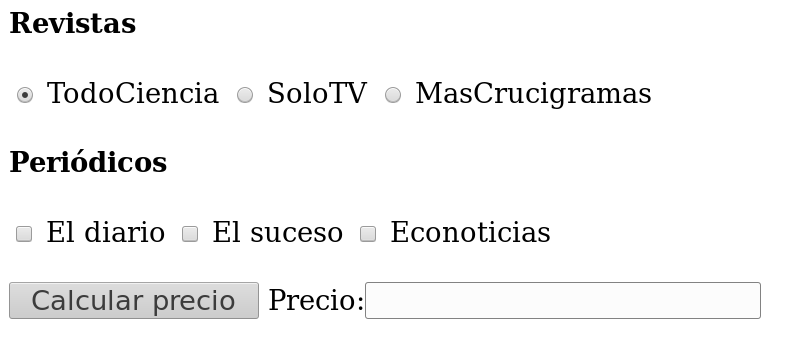
\includegraphics[width=.8\textwidth]{examen-img/revistas.png}
\caption{Formulario de compra editorial}
\end{figure}

\break

\begin{verbatim}
<!-- HTML con los controles-->
<h4>Revistas</h4>
<input type="radio" name="revistas" value="ciencia" id="ciencia" checked>

<label for="ciencia">TodoCiencia</label>
<input type="radio" name="revistas" value="tv" id="tv">

<label for="tv">SoloTV</label>
<input type="radio" name="revistas" value="crucigramas" id="crucigramas">
                   
<label for="crucigramas">MasCrucigramas</label>

<h4>Peri�dicos</h4>

<input type="checkbox" name="periodicos[]" id="diario" value="diario" >
<label for="diario">El diario</label>
                    
<input type="checkbox" name="periodicos[]" id="suceso" value="suceso">
<label for="suceso">El suceso</label>
                    
<input type="checkbox" name="periodicos[]" id="econoticias" value="econoticias">
<label for="econoticias">Econoticias</label>
<input type="submit" value="Calcular precio" onclick="calcular(); return false;">
Precio:<input type="text" id="precio_total">
\end{verbatim}
\end{document}
